\section{Introduction}
    Many algorithms exist to solve the problem of path planning—the problem of finding a path
    from a starting position to a goal position in some environment with obstacles. However,
    most of these algorithms involve expensive calculation and are not suitable for environments
    with moving obstacles. Some works are thus exploring methods of applying deep reinforcement
    learning (DRL) to the problem (TODO: reference other works). This work details one such
    method to apply DRL algorithms for path planning that relies only on a small patch of the
    environment at each time step to operate.

\section{Methodology}
    Our method is based on Deep Deterministic Policy Gradient (DDPG)
    \cite{DBLP:journals/corr/LillicrapHPHETS15} and allows an agent to make continuous movements
    within a grid environment. DDPG, like many other deep reinforcement learning algorithms,
    relies on three main components: \textit{states}, \textit{actions}, and \textit{rewards}.
    In this work, we refer to these components at time step $t$ as $s_t$, $a_t$, and $r_t$
    respectively.

    Note that we imagine the agent as mobile, so by the agent's current position we mean the
    position of the theoretical mobile device that would be performing the navigation.
    Simultaneously, we use the term agent in the traditional reinforcement learning sense:
    an intelligent algorithm that determines which actions to take given some state of the
    environment.

    During each time step, the agent is presented with a local view of its surroundings, with
    which it determines its immediate trajectory in order to avoid obstacles and reach the
    goal position. The following sections detail the environment setup, states, actions, and
    rewards used in the method.

    \subsection{Environment Setup and State}\label{sec:env_setup_state}
        The environment setup was kept as simple as possible to allow the agent to be extended
        to as many different applications as possible (e.g. UAVs, land robots, etc.). Hence, an
        environment is described as a 2-dimensional grid of spaces, each either traversable or
        not, representing a top-down view of the area of interest. Such an environment is stored
        as an image and some examples can be seen in Figure \ref{fig:environments}.

        At time step $t$, the state $s_t$ is a combination of 1) a local patch of the environment
        centered around the agent's current position and 2) the normalized displacement vector
        of the goal from the agent's current position.

        The local patch component of the state is a $11 \times 11$ grid space view of the
        environment centered at its current position. Since the agent may not be positioned at
        the exact center of a grid space, we perform bilinear interpolation to scale the weights
        of each component of this local view (see Figure \ref{fig:patch_view}).

        \begin{figure}[H]
        \centering
            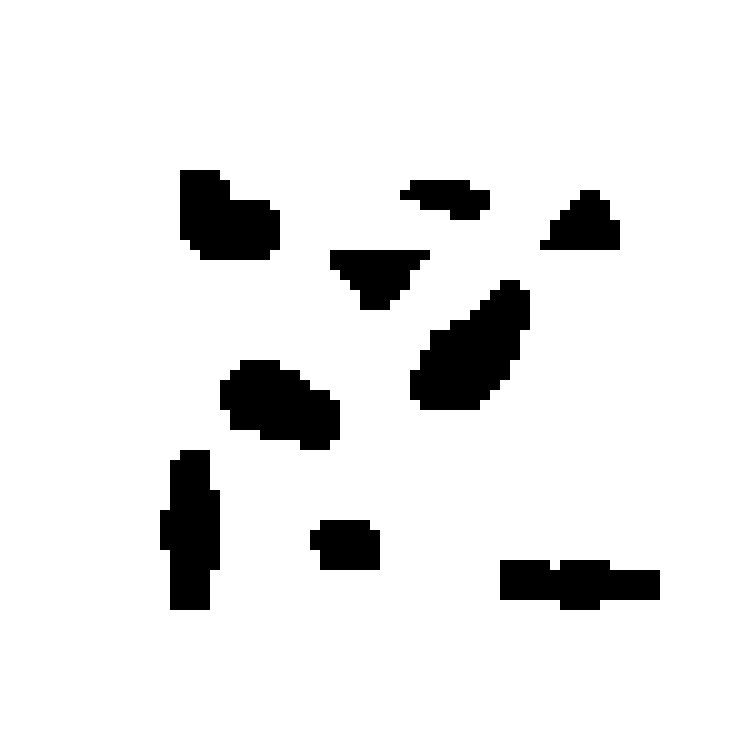
\includegraphics[width=2.75cm,frame]{grid4.png}
            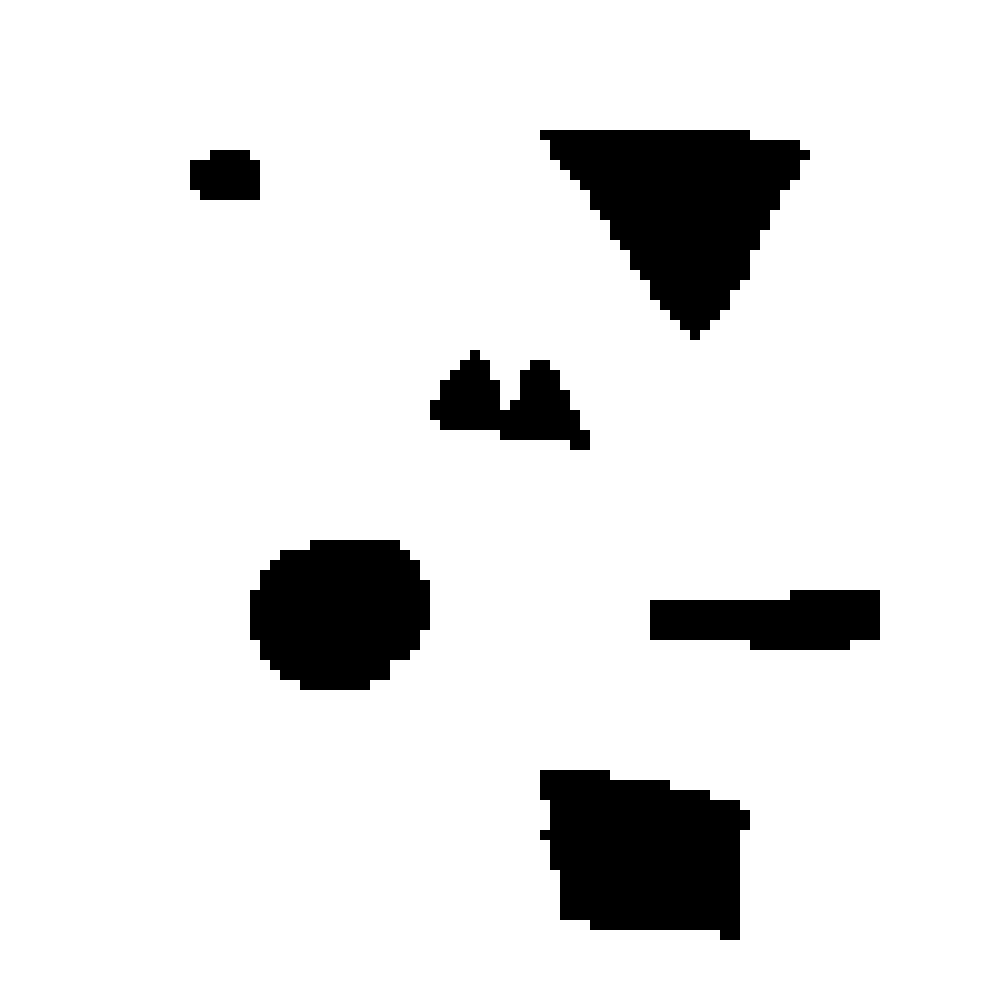
\includegraphics[width=2.75cm,frame]{grid3.png}
            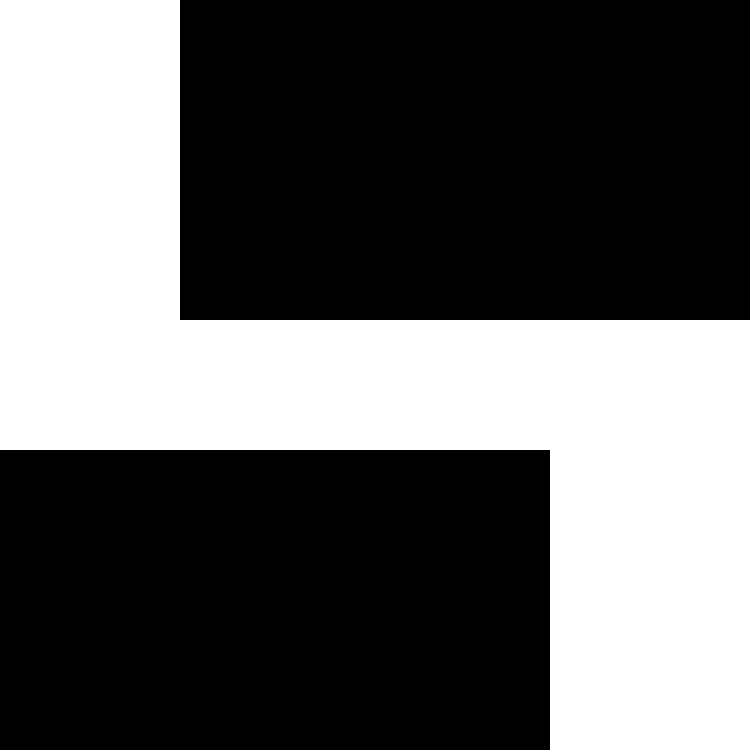
\includegraphics[width=2.75cm,frame]{grid5.png}
            \caption{Environments used for training and testing. Black pixels represent
                     an untraversable grid space, while white ones are traversable.}
            \label{fig:environments}
        \end{figure}

        \begin{figure}[H]
            \centering
                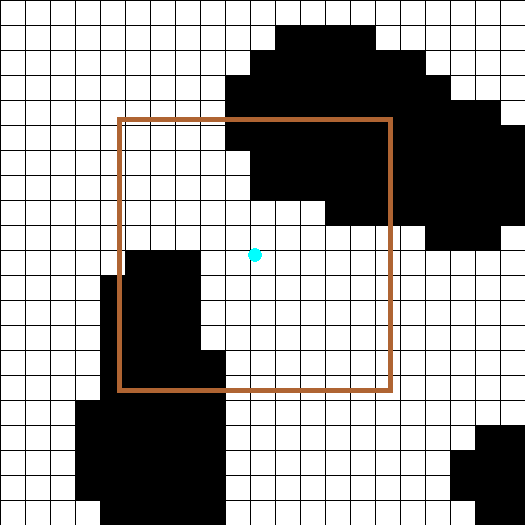
\includegraphics[width=4.25cm,frame]{patch_big.png}
                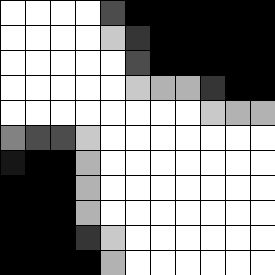
\includegraphics[width=4.25cm,frame]{patch_interp.png}
                \caption{Example of the bilinear interpolation of the agent's local view of
                         the environment. On the left the orange box represents the area of
                         the bigger environment that the agent can see, and on the right is
                         the interpolated view that the agent receives as input.}
                \label{fig:patch_view}
        \end{figure}

    \subsection{Agent Action Space}\label{sec:action_space}
        While the environment is defined within a uniform grid, the agent's action space is
        continuous. Hence, at time step $t$, the action $a_t \in \mathbb{R}^2$ is the velocity
        vector of the agent in 2-dimensional space.

        When the agent provides action $a_t$, we perform collision detection to ensure the agent
        cannot move through untraversable grid spaces.

    \subsection{Reward Functions}
        In this work, the reward function $r_t$ consists of a few components that encode
        certain behaviors we desire from a well-trained agent. These components are $r_{goal}$,
        $r_{dist}$, and $r_{margin}$. The component $r_{goal}$ is a constant reward given
        when the agent reaches the goal position.
        
        The component $r_{dist}$ is a function of the distance of the agent from
        the goal position. It is defined exactly as
        \begin{equation}
            r_{dist} = -C_1 d_{goal}
        \end{equation}
        where $C_1$ is a hyper parameter and $d_{goal}$ is the distance between the agent and
        the goal position. This function incurs a penalty for every simulation step, but this
        penalty shrinks as the agent approaches the goal. Hence, it encourages the agent to
        reach the goal in as few steps as possible.

        The component $r_{margin}$ is a function of the distance to the closest untraversable
        grid space from the agent, defined as
        \begin{equation}
            r_{margin} =
                \begin{cases}
                    -C_2(d_{wall}+0.5)^{-C_3} & \text{if $d_{wall} <= 6$} \\
                    0 & \text{if $d_{wall} > 6$}
                \end{cases}
        \end{equation}
        where $C_2$ and $C_3$ are hyper parameters and $d_{wall}$ is the distance between the
        agent and the closest untraversable grid space. This function was chosen because the
        penalty for the agent traversing close to an obstacle grows exponentially. Hence, it
        incurs a large penalty for collisions while still allowing the agent to traverse
        relatively close to obstacles without as much penalty.

        Finally, the total reward is defined as
        \begin{equation}
            r_t = r_{margin} + r_{dist} +
                \begin{cases}
                    r_{goal} & \parbox[t]{.45\columnwidth}{if the agent reached the goal in this
                                                          time step} \\
                    0        & \text{otherwise}
                \end{cases}
        \end{equation}
        where $r_{goal}$ is another hyper parameter.

    \subsection{Agent Network Structure}
        DDPG is an actor-critic deep reinforcement learning method, meaning our agent consists
        of two networks: the actor network that chooses actions based environment state, and
        the critic network that evaluates the Q-value of a given state and action pair.

        Our actor network takes the environment state (as described in Section
        \ref{sec:env_setup_state}) and produces an action $a_t$ (as described in Section
        \ref{sec:action_space}). The network architecture consists of 2D convolutional layers,
        followed by fully connected layers, with the final layer having a $tanh$ activation
        to clamp the velocity components in the range $(-1,1)$. See Figure
        \ref{fig:actor_network} for a detailed view of the network.

        The critic network is in many ways similar to the actor network, except the output
        is a single number (the Q-value) with a linear activation. See Figure
        \ref{fig:critic_network} for the detailed view.

        \begin{figure}[H]
            \centering
                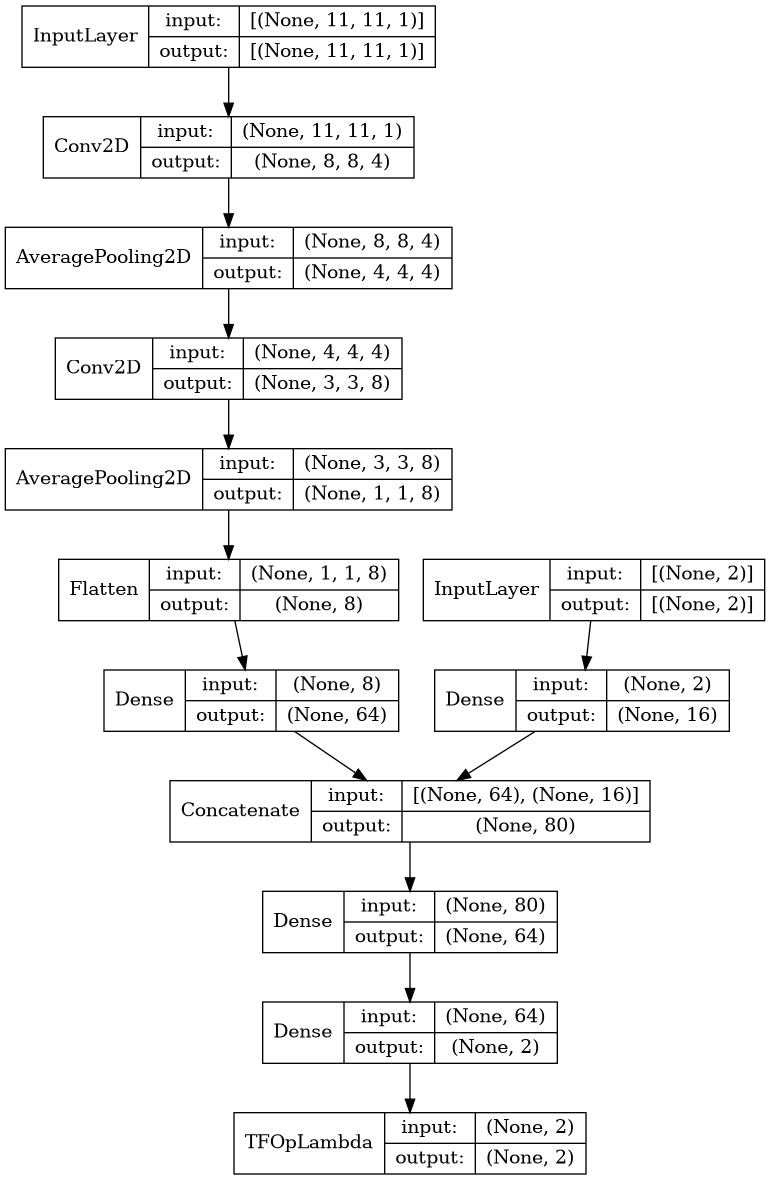
\includegraphics[width=6cm]{actor_model.png}
                \caption{Architecture of the actor network. TODO: Create better graphic.}
                \label{fig:actor_network}
        \end{figure}        

        \begin{figure}[H]
            \centering
                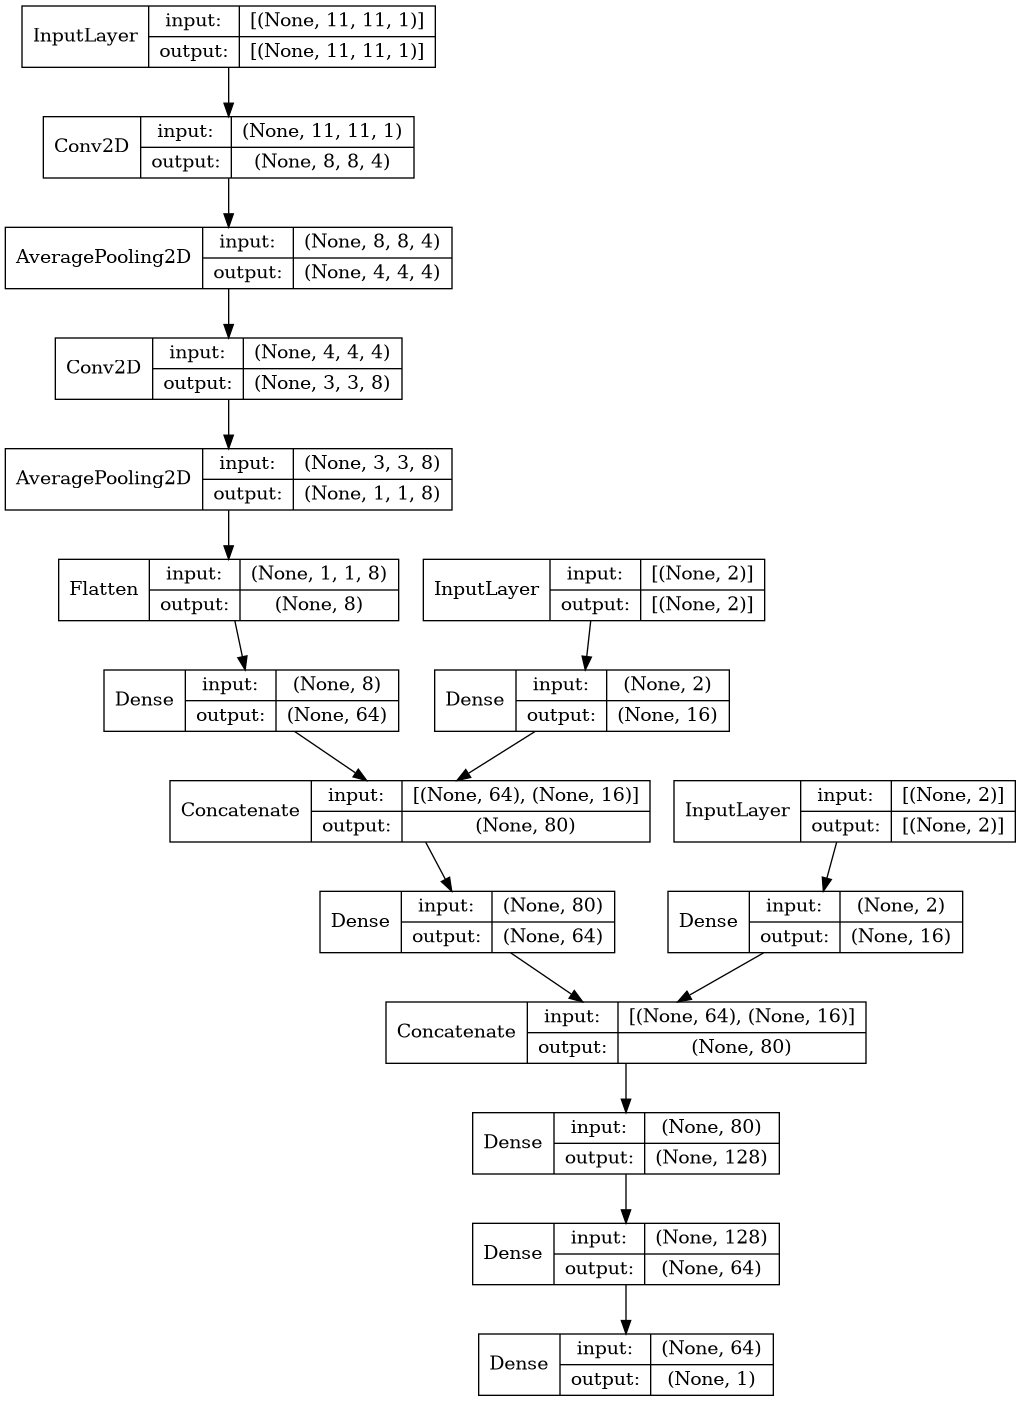
\includegraphics[width=6cm]{critic_model.png}
                \caption{Architecture of the critic network. TODO: Create better graphic.}
                \label{fig:critic_network}
        \end{figure}

    \section{Experiment Results}
        Our networks were trained using DDPG in an environment with many obstacles (the
        left-most environment shown in Figure \ref{fig:environments}). For each episode
        of training, the start and end states within the environment were randomized, taking
        care to not place either within or too close to an obstacle. Then, the agent
        uses its actor network to take steps through the environment. An episode ends when
        either the agent reaches the goal or a fixed number of time steps occur.

        After the agent was proficient in the training environment, its performance was evaluated
        in the other two environments of Figure \ref{fig:environments}. We evaluated the agent's
        performance with and without the $r_{margin}$ reward component, finding that the margin
        allowed for smoother traversal around obstacles. These results can be found in Figures
        \ref{fig:results_no_margin} and \ref{fig:results_with_margin}.

        \begin{figure}[H]
            \centering
                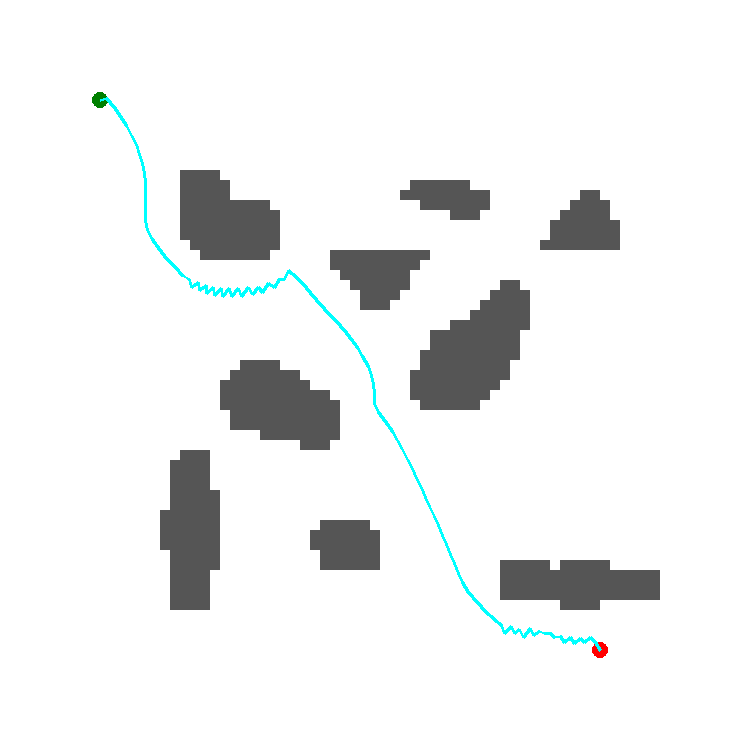
\includegraphics[width=2.75cm,frame]{continuous_grid4.png}
                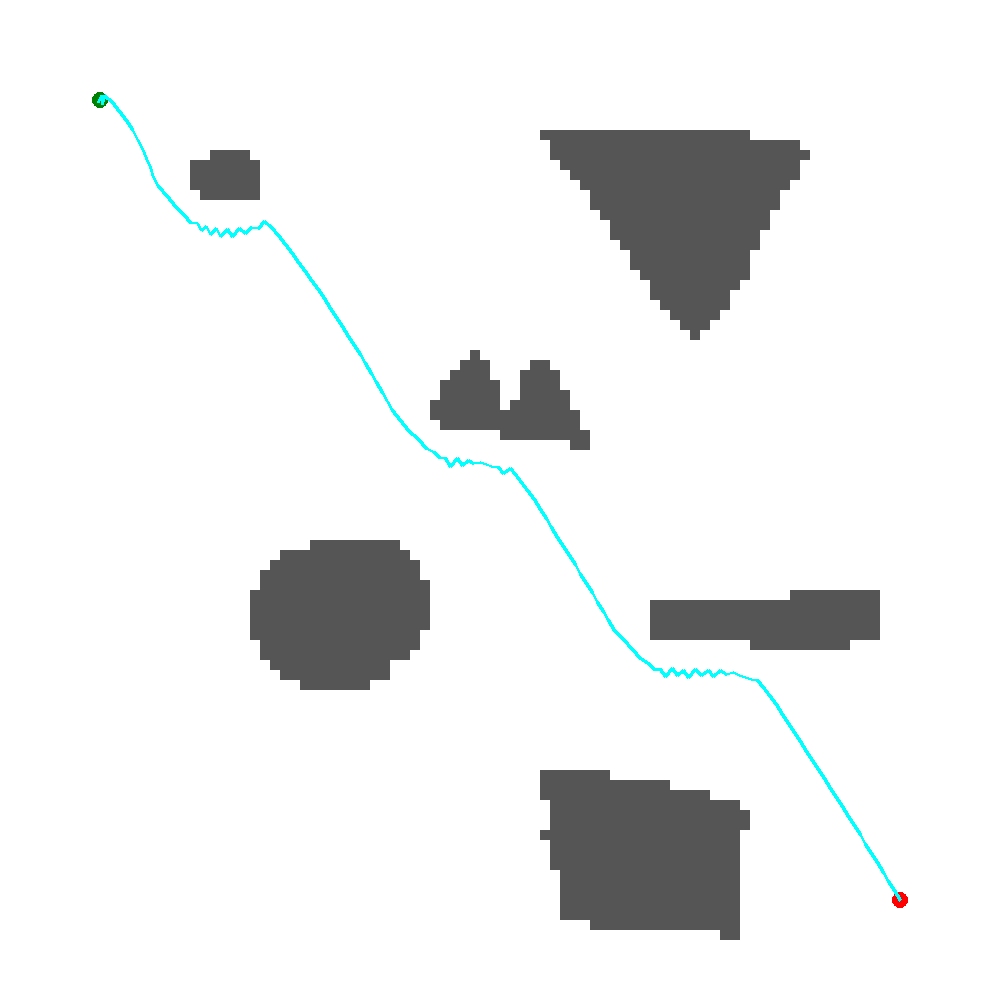
\includegraphics[width=2.75cm,frame]{continuous_grid3.png}
                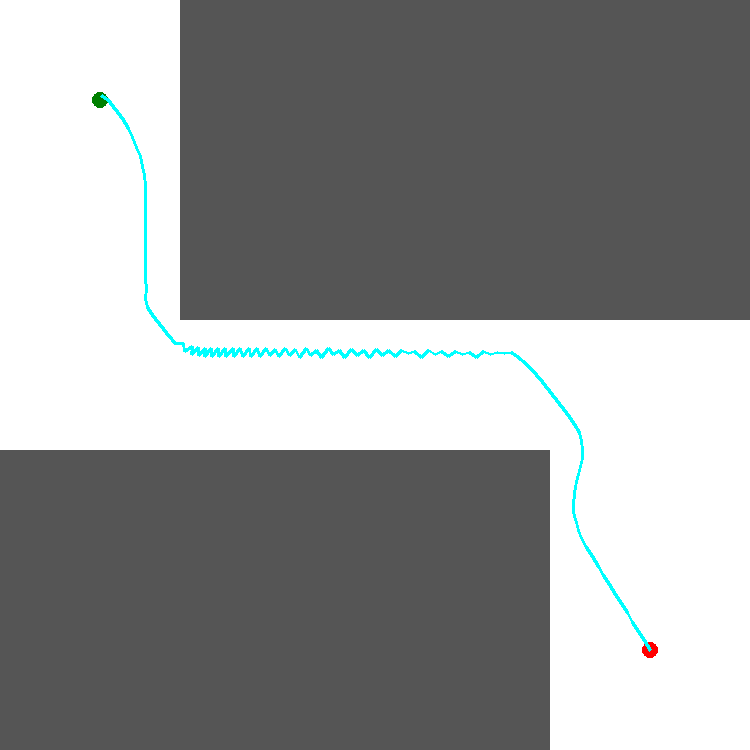
\includegraphics[width=2.75cm,frame]{continuous_grid5.png}
                \caption{Paths found \textit{without} the $r_{margin}$ reward component. The agent was
                         trained on the leftmost environment. The results for the right two
                         are generalization; the agent never saw these environments in training.}
                \label{fig:results_no_margin}
        \end{figure}

        \begin{figure}[H]
            \centering
                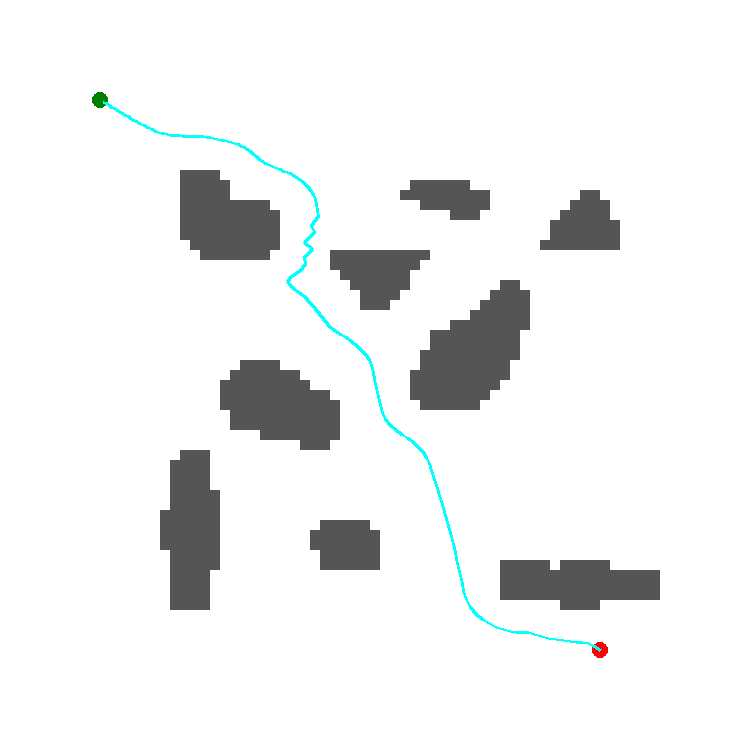
\includegraphics[width=2.75cm,frame]{new_grid4.png}
                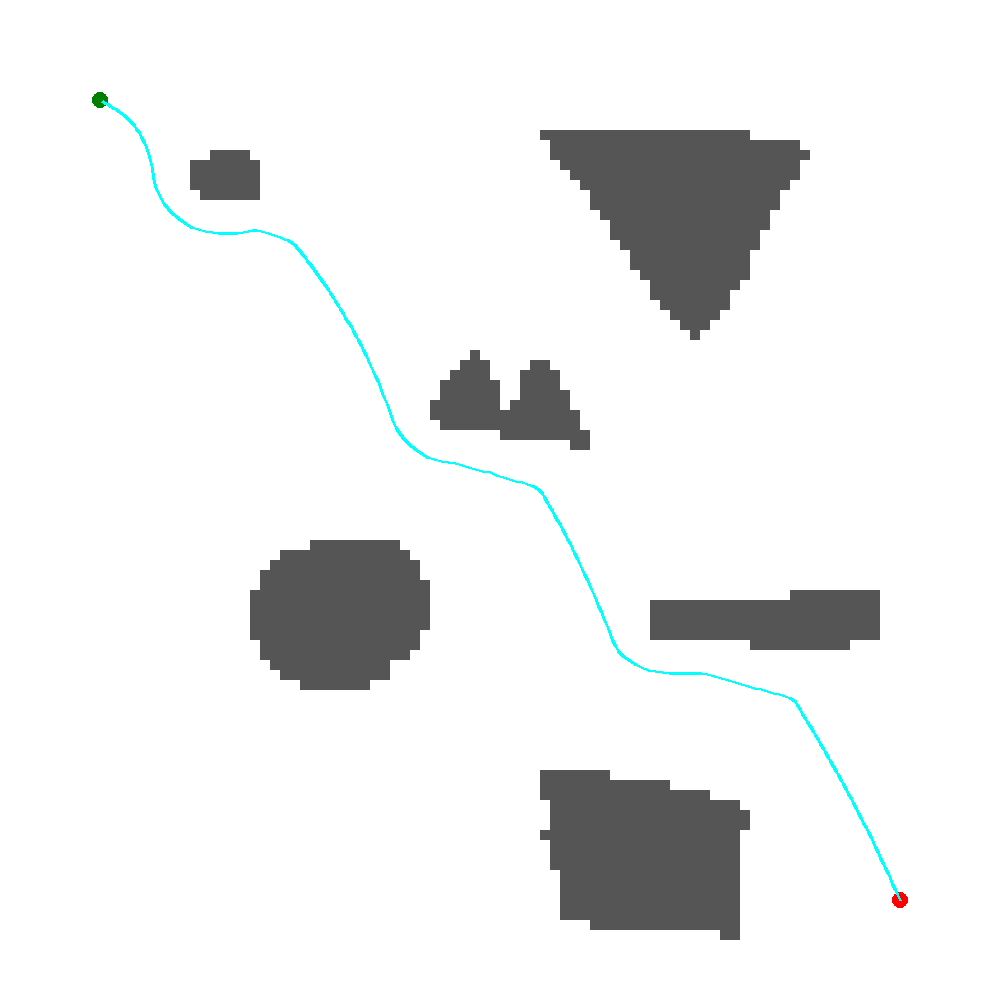
\includegraphics[width=2.75cm,frame]{new_grid3.png}
                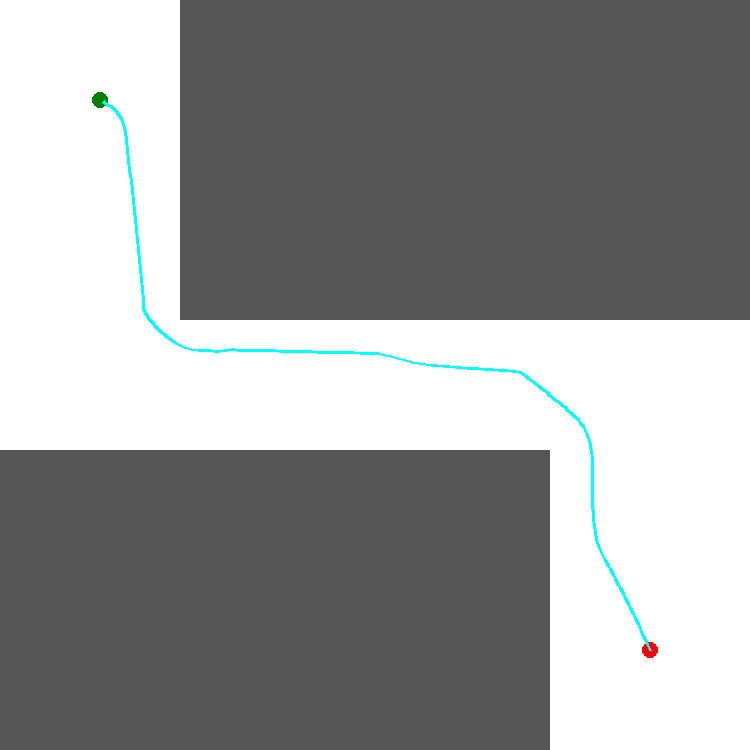
\includegraphics[width=2.75cm,frame]{new_grid5.png}
                \caption{Paths found \textit{with} the $r_{margin}$ reward component. The agent was
                         trained on the leftmost environment. The results for the right two
                         are generalization; the agent never saw these environments in training.}
                \label{fig:results_with_margin}
        \end{figure}

        TODO: Re-run some the experiments and get reward graphs over time.

    \section{Conclusion}
        This work presents a method of applying DRL algorithms to the task of path planning.
        From our empirical results, we find that such a method can be very effective for
        environments with simple obstacles. Furthermore, we find that our trained agents
        generalize well to new environments that were not encountered while training. We continue
        to develop this method, namely exploring more components to the reward function to further
        smooth the generated path.
